Este capítulo tem por objetivo detalhar os aspectos do desenvolvimento
do protótipo. Sua mecânica, funcionamento, decisões tecnológicas,
diagramas, entre outros aspectos serão tratados aqui.

\section{Mecânica}

Para a análise prática das limitações foi escolhido um jogo de
matemática simples. Consistindo na geração de equações cada qual 
com uma resposta candidata. Cabe ao usuário informar se o resultado apontado
pelo jogo está correto ou não. A cada resposta dada o nível de
complexidade da equação cresce. O tempo é um fator determinante
no resultado do jogo pois quão mais rápido o jogador acertar se a
afirmação está correta ou não mais pontos ele receberá. Esta
categoria de jogo foi selecionada por ter profundidade, oferecendo a
possibilidade de explorar diversos recursos do HTML, e criar melhorias
incrementais. E também por oferecer uma dificuldade técnica não
tão desafiadora visto que não disponho de experiência profunda no
desenvolvimento de jogos em geral.

Jogos como o Math Workout e o Countdown para Android tem uma temática
similar. Conquanto, o Math Workout não apresenta a resposta, sendo o
papel do usuário computar a equação e digitar o resultado. Já o jogo
Countdown apresenta um número final e requer que o usuário determine
a equação que resultou no valor à partir de um dado conjunto de
números e operadores. O jogo desenvolvido para o protótipo parece ter
uma melhor jogabilidade em dispositivos móveis que ambos os jogos acima
citados pois não requer a presença de um teclado numérico. Os botões
de verdadeiro ou falso contém todas as possibilidades de interação
com a aplicação. A figura \ref{fig:gameScreen} demonstra a interface
contendo os botões descritos.

\begin{figure}[H]
    \centering
    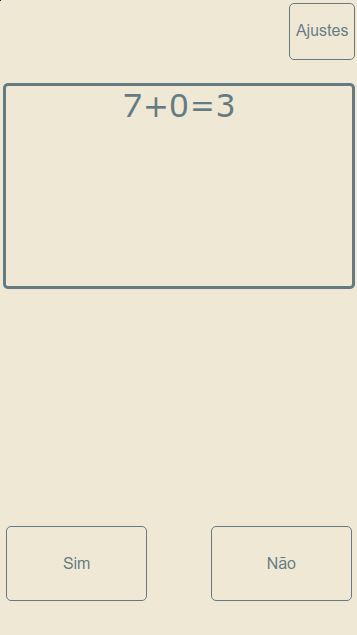
\includegraphics[height=10cm]{board.png}
	\caption{Interface do jogo com equação sendo apresentada}
    \label{fig:gameScreen}
\end{figure}

\section{Requisitos}

Abaixo estão detalhados os requisitos que uma mecânica como a descrita
acima deve prover.

\subsection{Requisitos funcionais}

\noindent As funcionalidades requeridas para o jogo são as seguintes:

\begin{itemize}
    \item O sistema deve prover equações matemáticas de dificuldade crescente para o usuário informar se estão corretas ou não;
    \item O sistema deve pontuar as respostas dadas com maior agilidade com uma pontuação maior que as respondidas com menor agilidade;
    \item O sistema deve apresentar a colocação da partida do usuário em comparativo com seu histórico.
\end{itemize}

\subsection{Requisitos não funcionais}

\noindent Outros aspectos requisitados mas que não fazem parte da regra de negócio:

\begin{itemize}
    \item O sistema deve ser desenvolvido utilizando as ferramentas da web.
    \item O sistema deve funcionar para a plataforma desktop e Android.
    \item O sistema deve ser desenvolvido sem a utilização de nenhuma biblioteca ou framework.
\end{itemize}

\section{Modelagem}

A figura \ref{fig:simpleDiagram} apresenta o diagrama de classes
simplificado \footnote{Nos anexos pode-se encontrar a versão completa
do diagrama de classes}.

\begin{figure}[H]
    \centering
    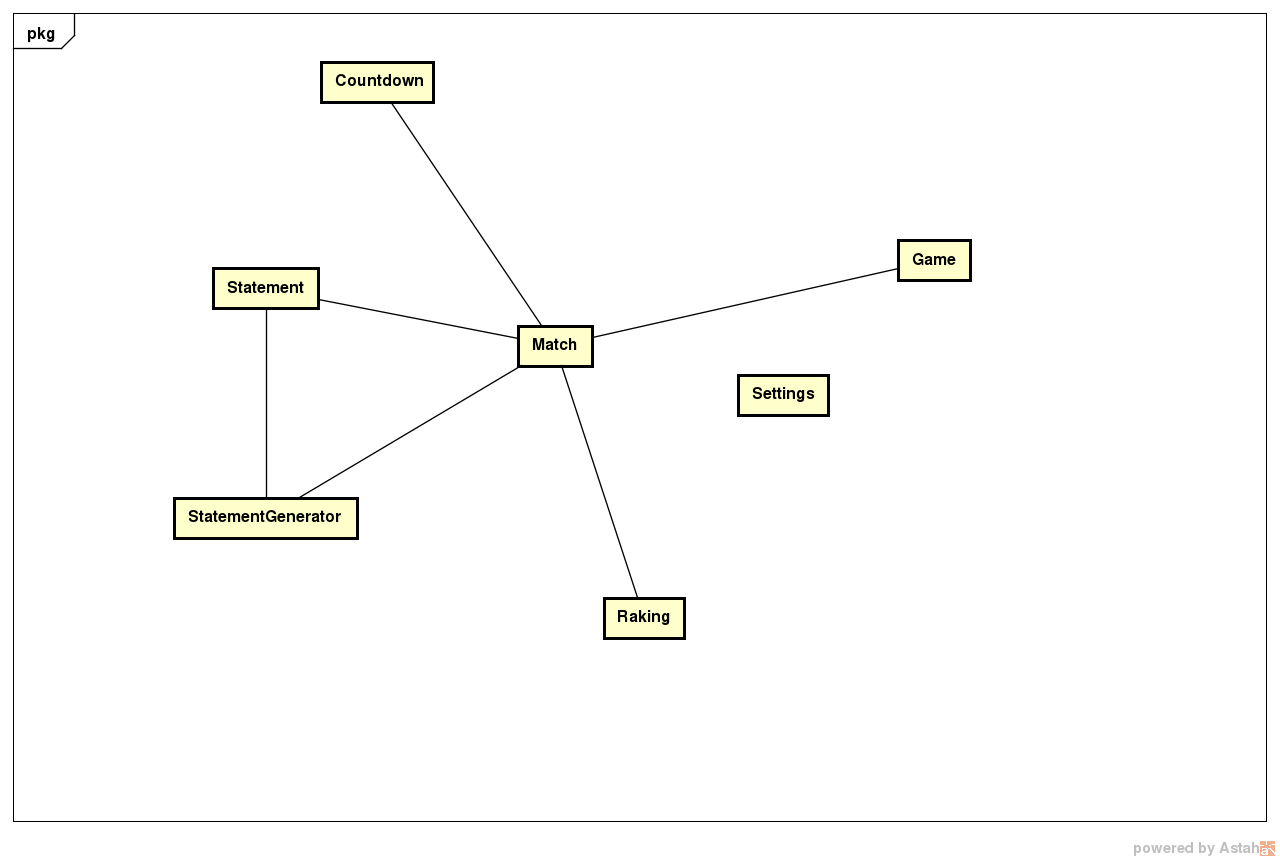
\includegraphics[width=0.8\textwidth,natwidth=610,natheight=642]{ClassesSimpleView.png}
	\caption{Diagrama de classes simplificado}
    \label{fig:simpleDiagram}
\end{figure}

\section{Desenvolvimento}

O desenvolvimento se deu com uma postura de melhoria progressiva
criando primeiramente  a versão mais simples possível para atingir as
requisitos funcionais. A partir dessa versão, novos recursos foram
sendo adicionados para melhorar a experiência do usuário. Iniciei o
desenvolvimento criando para a plataforma Desktop pois esta contém
um grande número de ferramentas de desenvolvimento nativas que não
requerem especial configuração.

O primeiro passo foi a criação do documento HTML, foram utilizados
elementos \textit{div} para simbolizar telas do jogo. Conter todas as
telas em único HTML caracteriza o jogo como uma aplicação de uma
única página (\textit{Single Page Application}). Alternativamente,
poderia se depender de um servidor para mandar as páginas prontas,
mas isso distribui a complexidade do sistema para tecnologias do
lado do servidor, distanciando-se da proposta de um jogo construído
exclusivamente com as tecnologias da Web.

Seguindo a construção do documento HTML veio o desenvolvimento de um
CSS simples que comporta a visualização em múltiplos dispositivos.
Para tal, foram utilizadas posições e tamanhos relativos. Por exemplo,
a largura de cada tela da SPA é 98\% do tamanho total disponível no
dispositivo. Já o tamanho da fonte do quadro principal, representado
pelo id \textit{billboard}, é duas vezes o tamanho da fonte normal (2em).
Sem a ajuda de bibliotecas especializadas o processo de criação da
interface não é trivial. Apesar da interface ser simples, fazer os elementos
se alinharem em diversos tamanhos de telas não é fácil e pode se
tornar um problema substancial para interfaces realmente complexas.
A figura \ref{fig:gameScreen} e \ref{fig:gameScreenDesktop} apresentam
a tela principal do jogo em um dispositivo móvel e em um desktop, respectivamente.

\begin{figure}[H]
    \centering
    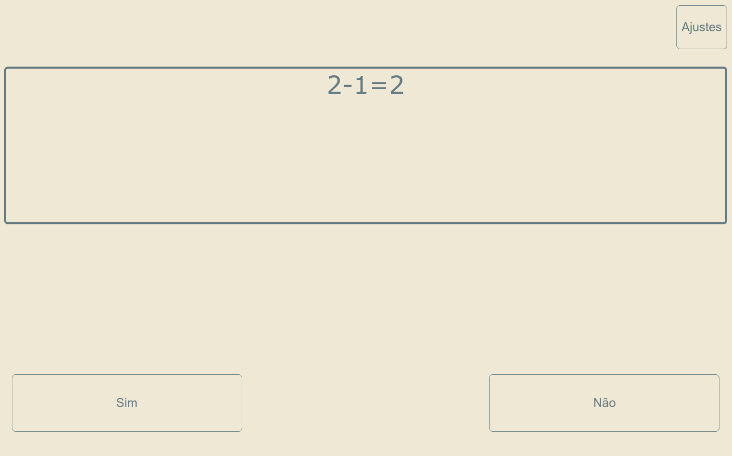
\includegraphics[height=9cm]{board-desktop.png}
	\caption{Interface do jogo com equação sendo apresentada no desktop 1440x900}
    \label{fig:gameScreenDesktop}
\end{figure}

Após a concepção do CSS deu-se início ao desenvolvimento da lógica
das páginas em JavaScript. O primeiro passo consistiu em habilitar o
funcionamento de múltiplas telas em um único arquivo HTML através
de JavaScript. Os botões que levam a outras telas, quando clicados,
simplesmente escondem todas as seções e por fim carregam a que estão
configurados para mostrar.

Aplicativos SPA introduzem outros desafios. Por exemplo, o botão
de voltar perde sua utilização, visto que não se está trafegando
de uma página a outra, somente em partes de uma mesma página. HTML5
provê uma API em JavaScript para manipular o histórico que pode
resolver este problema; entretanto, no protótipo não adicionamos
esta funcionalidade pois a quantidade de telas é realmente baixa e os
benefícios introduzidos seriam pequenos.

Ao iniciar a execução do JavaScript todas as \textit{divs} que
representam telas são escondidas e a \textit{div} de carregamento de
recursos é mostrada em seguida. O objetivo desta \textit{div} é não deixar
o usuário sem feedback enquanto os recursos necessários para a
utilização do jogo não estão disponíveis. Todavia, o carregamento
é realmente rápido e o usuário, a não ser que dependa de uma rede
muito lenta, geralmente não vê a tela. No final do carregamento
de todos os recursos é disparado o evento \textit{window.onload},
neste momento carrega-se a \textit{div} da partida e dá-se início a mesma.
Durante esta fase do desenvolvimento também foram adicionados
\textit{listeners} aos demais elementos interativos do jogo, como
clicar nas configurações e nos botões de certo e errado da página
principal. Deixando a página pronta para receber a funcionalidade
propriamente dita.

Com esqueleto da aplicação definido foi introduzida a lógica
de negócio. A figura \ref{fig:simpleDiagram} apresenta a
relação entre as classes do jogo. De toda a regra do jogo, a classe
\textit{Match} é a mais importante. Ela simboliza uma partida dentro
do jogo, é na classe \textit{Match} que as informações de quantas
equações existem, quantas foram acertadas, o tempo total da partida,
bem como a pontuação atual do usuário são armazenadas. A cada
iteração do laço do jogo uma nova pergunta é dada pela classe
\textit{Match} e espera-se por uma resposta. Quando a resposta é dada
a classe \textit{Match} computa se ela está correta ou não e
o tempo que levou para chegar ao resultado. Quando não existem mais
perguntas para serem processadas é lançado um evento de final de
partida onde o resultado pode ser processado pelas demais classes do
jogo.

O cálculo da pontuação se dá por uma operação matemática simples.
Ao final de uma partida é computado o total de questões acertadas,
multiplicado por dez, divido pelo total de respostas, menos o total de
respostas certas adicionando-se 20\% do tempo da duração em segundos.
A figura \ref{fig:punctuationCalculation} apresenta o código utilizado
para o cálculo acima descrito.

\begin{figure}[H]
\centering
\begin{verbatim}
parseInt(
(this.rightAnswered * 10 ) / (
    (this.answersTotal - this.rightAnswered) 
    + (this.duration*0.2))
)
\end{verbatim}
\caption{Cálculo da pontuação do jogador}
\label{fig:punctuationCalculation}
\end{figure}

A construção da classe \textit{Match} disponibilizou o comportamento
principal do jogo; entretanto, nesta etapa não havia um gerador de
equações. O jogo contava apenas com uma coleção de equações
preestabelecidas que eram selecionadas aleatoriamente a cada turno.
Adiar a construção do gerador de equações se provou uma boa
escolha pois possibilitou que o desenvolvimento se focasse em outros
aspectos importantes, como a elaboração do laço do jogo, ranking,
configurações, entre outros.

O ranking serve para armazenar o resultado de cada partida do jogador
possibilitando uma percepção de histórico de performance. Os
dados são armazenados em Local Storage, escolhido por ter uma API
simples. Arquiteturalmente falando, IndexedDb se encaixaria bem na
aplicação por ter uma interface chave valor, ideal para um ranking,
onde as chaves poderiam ser as posições do usuário. Entretanto, a
interface totalmente orientada a eventos do IndexedDb introduz uma
camada de complexidade desnecessária para os casos simples. Por
conseguinte, visto que os requerimentos do protótipo não demandam
grande performance ou armazenamento massivo de dados, a opção
modesta, Local Storage, foi preferida. A classe ranking é simplesmente
uma interface para converter partidas e armazenar e recuperar estas
informações em Local Storage. A figura \ref{fig:placar} demostra
as informações do resultado de uma partida bem como a posição do
ranking.

\begin{figure}[H]
    \centering
    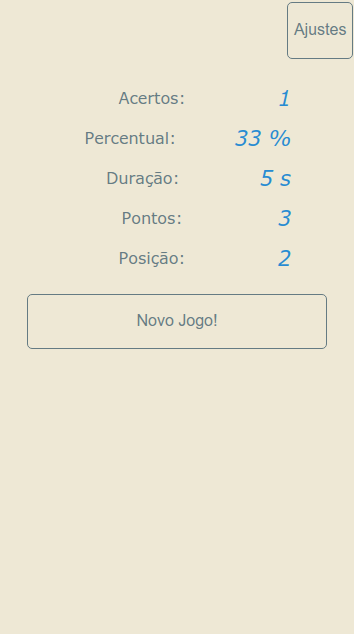
\includegraphics[height=10cm]{score.png}
	\caption{Resultado de uma partida}
    \label{fig:placar}
\end{figure}

O objeto \textit{Settings}, assim como o Ranking, utiliza Local Storage
e provê uma interface para armazenar e recuperar preferências sobre
o jogo. Cada campo editável na tela de configurações contém
\textit{listeners} prontos para registrar no objeto \textit{Settings}
cada mudança que ocorrer em seus estados. Os objetos que utilizam estas
configurações também o fazem através do objeto Settings, nunca
acessando configurações diretamente em Web Storage. Dessa forma a
validade das configurações é garantida e a migração para uma forma
de armazenamento diferente é possível com relativa facilidade.
A figura \ref{fig:configurations} demonstra a tela de configurações do 
jogo.

\begin{figure}[H]
    \centering
    
\includegraphics[height=10cm]{settings.png}
	\caption{Configurações do jogo}
    \label{fig:configurations}
\end{figure}

Implementados estes mecanismos essenciais para o jogo, pude me focar no
ponto central do negócio e possivelmente o mais complexo: a geração
de equações. A geração das equações é feita randomicamente e
envolve duas classes: \textit{Statement} e \textit{StatementGenerator}.
O objeto \textit{Statement}, é responsável por armazenar as
informações de uma equação, à dizer: a afirmação sendo feita
e se seu resultado está correto ou não (a reposta da afirmação).
O objeto \textit{StatementGenerator} é responsável por gerar
instâncias da classe \textit{Statement}.

A classe \textit{StatementGenerator} conta com um método
\textit{getStatement} que realiza o processamento para gerar um novo
\textit{Statement}. Esta função recebe como argumento um inteiro que
simboliza a dificuldade da equação. A cada resposta dada pelo usuário,
armazenada no objeto \textit{Match}, a dificuldade é incrementada
e repassada para o gerador. O valor da dificuldade é utilizado
internamente no \textit{StatementGenerator} para selecionar qual
operador será utilizado e o tamanho do multiplicador dos números
que compõem as equações. Para colocar claramente: as equações
são geradas através da randomização de valores e operadores (com
suas respectivas dificuldades processadas). Segue-se com a execução da
equação para determinar seu resultado e a geração, em 50\% dos
casos, de um valor errado de modo que a resposta não seja sempre
correta.

O objeto \textit{StatementGenerator} reside como membro de classe de
\textit{Match} e a cada interação com o usuário uma nova equação
é gerada por ele e armazenada no atributo \textit{currentStatement}
do objeto \textit{Match}. Ao final das iterações com o usuário o
evento \textit{endOfMatch} é lançado onde os pontos são computados,
armazenados e mostrados para o usuário. Neste ponto é possível
começar outra partida reiniciando o processo.

Estas classes comportam os requisitos funcionais do jogo. Entretanto,
após um período de uso, foi identificado que muitas vezes o usuário
começa uma partida e não está prestando atenção na tela o
que acarreta na perda de pontos no período inicial da partida. Para
reduzir este problema foi adicionada a classe \textit{Countdown},
que é basicamente um temporizador regressivo que demarca o início
de cada partida, notificando o usuário quanto falta para a partida
iniciar. O temporizador foi desenvolvido em canvas e apresenta 4
demarcações desenhadas a cada 90 graus, formando um circulo com uma
mensagem no centro, neste caso os números do temporizador. A figura
\ref{fig:counter} demonstra o contador prestes a iniciar uma nova
partida.

\begin{figure}[H]
    \centering
    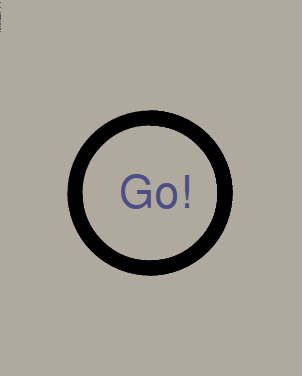
\includegraphics[height=10cm]{countdown.png}
	\caption{Contador em Canvas}
    \label{fig:counter}
\end{figure}

Para melhorar a experiência em desktops foram adicionados controles de
teclado além dos já presentes botões na interface, possibilitando que
o usuário utilize o teclado além do mouse. Quando o usuário utilizar
a seta para esquerda ou direita os botões Sim ou Não, respectivamente,
são clicados através de JavaScript. Simular o clique ao invés de
acionar duas vezes o tratamento das escolhas de resposta foi uma boa
estratégia pois centralizou o tratamento, evitando duplicação de
código.

Nos dispositivos móveis, com intuito de melhorar a experiência, foram
adicionadas vibrações para as respostas erradas. A API de vibração
é trivial e sua utilização possibilita uma experiência mais
profunda com a aplicação, sendo uma adição de bom custo/benefício.
Se o usuário desejar utilizar o mouse no desktop, foram adicionadas
transformações do CSS quando o ponteiro se encontra acima dos
botões. Para melhorar o feedback visual, os botões de certo e errado
tornam-se verdes ou vermelhos dependendo se o usuário acertou ou não
a questão dada. No quesito feedback auditivo foram adicionados sons
através da API de áudio do HTML para as respostas corretas e incorretas. Com estes
detalhes pormenorizados, fica visível que grande parte do tempo de
desenvolvimento de jogos multiplataforma é utilizado em fornecer uma
experiencia rica em interatividade, que faça uso das peculiaridades de
cada plataforma.

Durante o desenvolvimento foram utilizadas funções imediatamente
invocadas para declarar as classes. Isso se demonstrou uma boa forma
de separar os objetos, tornando o conflito de variáveis globais um
problema inexistente. Outro aspecto positivo foi a utilização de
um meta objeto para encapsular os demais, similar ao conceito de
\textit{namespaces}, neste caso utilizei o nome MyMath garantindo que
problemas de conflitos de nomes não aconteçam.

Ao final do desenvolvimento foi feita a integração do Grunt com
plugins de minificação de JavaScript e CSS \footnote{Para mais
informações sobre o Grunt veja os apêndices}. O grunt foi configurado
para disponibilizar a aplicação para distribuição dentro do
diretório \textit{dist/web}. Depois de a disponibilização Web estar
funcionando, foi feita a integração para o PhoneGap Build. Para
tanto foi utilizado um makefile que simplesmente copia os arquivos de
distribuição da Web, gerados pelo grunt, e o arquivo de metadados do
Phonegap Build, e cria a árvore de arquivos padronizada que o Phonegap 
Build requer.

\subsection{Performance}

A performance, mesmo sem otimizações ficou razoável. O tempo de
carregamento no Google Chrome desktop em uma rede 4G, comum no Brasil,
ficou em 1.4 segundos em média. Esta métrica foi extraída através da
ferramenta de depuração do Google Chrome que fornece a possibilidade
de simular a velocidades de redes.

Utilizado os arquivos minificados, gerados pelo Grunt, o tempo médio
de carregamento ficou em 1.1 segundos. Uma diferença substancial dada a
quantidade pequena de arquivos minificados (8 arquivos JavaScript e um
arquivo CSS).

A seguir serão tratadas algumas otimizações para jogos descobertas
através do desenvolvimento e pesquisa bibliográfica deste trabalho.

\section{Otimizações para jogos} \label{optimizations}
%{{{
Navegadores tentam otimizar a experiência de navegação definindo
um conjunto de regras e configurações razoáveis para a maioria dos
casos. Não obstante, nem sempre estes valores padrões são as melhores
opções no contexto de jogos. Abaixo seguem algumas otimizações
nas tecnologias da Web, direcionadas aos jogos, que foram identificadas
através da revisão e desenvolvimento do protótipo.

\subsection{CSS}

Scroll é um recurso interessante para longas páginas de texto,
o mesmo não se pode dizer à respeito de jogos.
Principalmente aqueles dependente de contato com a tela, pois
no contato a tela pode mover-se e desconcentrar o usuário. Para
remover este comportamento deve-se utilizar o \textit{overflow:
hidden;} no seletor do corpo do documento (\textit{body}).

A barra de endereço é outro recurso de pouca utilidade no contexto
de jogos, e muitas vezes um empecilho para jogos em dispositivos
móveis, devido ao limitado tamanho da tela. Para desabilitar a barra em
dispositivos da Apple pode-se utilizar a seguinte configuração:

\begin{verbatim}
<meta name="apple-mobile-web-app-capable" content="yes" />
\end{verbatim}

Segundo \citet{homescreenwebapps} o Google Chrome, a partir da versão
31, adicionou suporte a esta notação, inclusive o prefixo Apple, mas
as intenções são que o prefixo seja removido nas próximas versões.
Para os demais dispositivos não existe meio oficial de esconder a
barra de endereço. No entanto, alguns sites recomendam a solução
descrita abaixo:

\begin{verbatim}
<body onload="setTimeout(function() {window.scrollTo(0, 1)}, 100)">
</body>
\end{verbatim}

Apesar de não fazer parte de nenhuma especificação, a maioria dos
navegadores implementa a possibilidade de desativar a seleção de texto
na tela. Em jogos essa possibilidade é útil, pois não é natural e
possivelmente frustrante selecionar texto ao tentar interagir com a
interface. \citet{html5mostwanted} cita que desabilitar a seleção de
texto em jogos é uma otimização importante para a experiência do
usuário. Para fazê-lo, pode-se utilizar as regras CSS demonstradas
abaixo.

\begin{verbatim}
-moz-user-select: none;
-webkit-user-select: none;
-ms-user-select: none;
\end{verbatim}

\subsection{JavaScript}

A seguir serão descritas algumas otimizações de JavaScript no
contexto de jogos.

\subsubsection{Modo estrito}

Um recurso interessante do JavaScript é seu modo estrito, este faz
um conjunto de modificação na semântica do interpretador de modo
que alguns recursos suportados, mas propensos a problemas, sejam
desabilitados. Um exemplo de sintaxe válida propensa a erros é a
utilização variáveis não prefixadas pela palavra chave \textit{var},
que torna as variáveis em variáveis globais.

O modo estrito pode ser entendido como uma variante mais rígida do
JavaScript. Este mecanismo pode ser habilitado utilizando o termo
\textit{"use strict;"} nos cabeçalhos de arquivos ou funções .
Este controle localizado permite que código não estrito trabalhe
em conjunto com código estrito, característica conveniente para a
utilização em sistemas legados.

\subsubsection{Funções imediatamente invocadas}

Um problema comum de sistemas complexos em JavaScript é que muitos
objetos vivem em ambiente global. Isso pode causar uma coleção de
problemas, desde conflitos de nomes à sobrescrita de variáveis. Para
contornar esse problema pode-se utilizar as funções imediatamente
invocadas IFE (\textit{Immediatly invoked function expression}).

\begin{figure}[H]
\centering
\begin{verbatim}
    (function() {
        'use strict';

        function bar() {
            return 'foo';
        }

        window.bar = bar;
    })();
    window.bar();
\end{verbatim}
\caption{Exemplo de função imediatamente invocada.}
\label{fig:iife}
\end{figure}

A figura \ref{fig:iife} demonstra a utilização deste padrão. As
funções definidas no mesmo nível que bar não estarão no contexto
global, a não ser que seja especificado diretamente, e não sofrerão
conflitos de nomes e outros problemas relativos ao contexto global.

Outro fator importante na construção de jogos em JavaScript é a
otimização do laço do jogo. Para escrever o laço é possível
utilizar as funções do JavaScript \textit{settimeout} ou
\textit{setInterval}. Não obstante, a forma mais recomendada é
utilizar a função \textit{requestAnimationFrame}. Esta função reduz
ou completamente desabilita a execução do laço enquanto o usuário está
em outra aba. Por conseguinte, o consumo de bateria é reduzido, uma
característica importante para dispositivos móveis.

\subsubsection{HTML}

Um problema que jogos em HTML sofrem é a demora no carregamento
da grande quantidade de recursos que geralmente precisam estar em
memória para o jogo funcionar. Muitos jogos utilizam uma tela de
carregamento enquanto os recursos são adquiridos. Existem algumas
formas de minimizar este problema, como utilização de cache, CDN's,
minificação, entre outros.

Uma funcionalidade do HTML interessante para otimizar o tempo de rede
o pré carregamento de recursos (\textit{Link Prefetching}). Esta
tecnologia possibilita que o navegador, em seu tempo livre, adquira
recursos que provavelmente serão necessários em um futuro próximo.

Nem todos os recursos necessitam ser pré carregados, mas uma impressão
muito superiora é criada se os recursos estão imediatamente
disponíveis quando uma nova fase é carregada \autocite[p. 39]{creatingFun}.
%}}}

A seguir serão apresentadas as limitações do HTML encontradas durante
o desenvolvimento do protótipo e pesquisa relacionada.

